% !TeX spellcheck = en_US
\documentclass[a4paper,10pt]{report}
\usepackage[a4paper,margin=2.5cm]{geometry}
\usepackage[british]{babel}
\hyphenation{GBARunner}
\usepackage{hyperref}
\usepackage{parskip}
\usepackage{enumitem}
\usepackage{multirow}
\usepackage{colortbl}
\usepackage{nicematrix}
\usepackage{hhline}
\usepackage{bytefield}
\usepackage{adjustbox}
\usepackage{makecell}
\usepackage{todonotes}
\usepackage{fontspec}
\usepackage[backend=bibtex]{biblatex}
\addbibresource{refs.bib}
\setmainfont{Arial}
\setmonofont{Consolas}
\title{GBARunner 3\\Technical Reference Manual}
\author{Gericom}
\date{26 August 2023}

% facilitates the creation of memory maps. Start address at the bottom, end address at the top.
% syntax: \memsection{end address}{start address}{height in lines}{text in box}
\newcommand{\memsection}[4]{
	\bytefieldsetup{bitheight=#3\baselineskip}    % define the height of the memsection
	\bitbox[]{10}{
		\texttt{#1}     % print end address
		\\ \vspace{#3\baselineskip} \vspace{-2\baselineskip} \vspace{-#3pt} % do some spacing
		\texttt{#2} % print start address
	}
	\bitbox{16}{#4} % print box with caption
}

\begin{document}
\maketitle
\tableofcontents
\chapter{Introduction}
	GBARunner 2 is a hypervisor that can run GBA games on the DS in DS mode. Because GBARunner 2 started out as a proof of concept and grew into a large project, it contains some fundamental design flaws and has become hard to maintain. GBARunner 3 is supposed to be the successor to GBARunner 2, attempting to improve its major flaws.
	
	The following points should be improved on project level:
	\begin{itemize}
		\item Compile properly with the latest devkitARM version (and not be dependent on a specific version in general);
		\item Natively support the DSi/3DS SD card;
		\item Better documented and maintainable code.
	\end{itemize}

	On a technical level the following points should be improved:
	\begin{itemize}
		\item Allow code to run, even if it is in higher parts of the rom that have not been linearly loaded into memory (also called hicode);
		\item Improve the sound emulation; in particular the direct sound channels and especially on regular DS devices;
		\item Have more control over the running game.
	\end{itemize}

	The following additional features were commonly requested for GBARunner 2 but were never realized:
	\begin{itemize}
		\item Cheat support;
		\item Save states;
		\item Sleep support; both when closing the lid and when selected ingame in supported games;
		\item Disabling the screen that is not being used to save battery.
	\end{itemize}

	In this document various new ideas for GBARunner 3 will be documented, together with lessons learned from GBARunner 2 and the things that already worked well.

\chapter{Implementation challenges}
\section{CPU compatibility issues}
	CPU compatibility issues exist because ARM7TDMI code is executed on an ARM946E-S core. While the ARM946E-S is backwards compatible in the defined behavior of instructions, its (in ARM terminology) unpredictable behavior (which means it depends on the CPU implementation) does differ to some extent. The following differences have been identified:
	\subsection{\texttt{LDR pc}, \texttt{LDM \{\dots,pc\}} \--- ARM/Thumb switching}
	In \texttt{LDR pc} and \texttt{LDM \{\dots,pc\}} instructions the ARM7TDMI ignores the thumb bit of the loaded address. By default the ARM946E-S switches between ARM and Thumb based on the lsb of the loaded value.
	
	\subsubsection{Impact}
	Only a small number of games depend on this behavior, including \textit{Final Fantasy IV} and \textit{Maya the Bee Sweet Gold}. It is likely that such games were compiled without interworking.
	
	\subsubsection{Solution}
	The behavior can be disabled in the CP15 control register for backwards compatibility purposes.
	
	\subsubsection{Impact of solution}
	Fixes the issue completely without any performance impact. Care should be taken to not depend on the ARM/Thumb switching behavior when the backwards compatibility mode is enabled. The compiler can for example generate a \texttt{POP pc} because it assumes it is safe to do on an armv5te processor.
	
	\subsection{\texttt{LDRH} \--- Unaligned behavior}
	When an \texttt{LDRH} is performed with an odd address the ARM7TDMI force-aligns, reads the 16-bit value at the aligned address and then rotates right by 8 bits similar to an unaligned \texttt{LDR}. For example if the bytes in memory look like \texttt{55 AA} and assume the unaligned address points to \texttt{AA}, the resulting value will be \texttt{0x550000AA}. The ARM946E-S still force-aligns, but the rotation no longer happens, resulting in \texttt{0x0000AA55}.
	
	\subsubsection{Impact}
	Unknown. Could effect a very small number of games, but can be game breaking. Aborted reads are not effected, because the memory emulation emulates the ARM7TDMI behavior.
	
	\subsubsection{Solution}
	Replace by an exception generating instruction and emulate.
	
	\subsubsection{Impact of solution}
	Impacts performance.
	
	\subsection{\texttt{LDRSH} \--- Unaligned behavior}
	On ARM7TDMI an unaligned \texttt{LDRSH} force-aligns, reads the 16-bit value at the aligned address, sign extends and then performs an additional arithmetic right shift of 8 bits. As such the resulting value is as if \texttt{LDRSB} was used (but I assume for the memory system it will still be a 16-bit access). For example if the bytes in memory look like \texttt{55 AA} and assume the unaligned address points to \texttt{AA}, the resulting value will be \texttt{0xFFFFFFAA}. The ARM946E-S still force-aligns but does not apply the extra shift, resulting in \texttt{0xFFFFAA55}.
	
	\subsubsection{Impact}
	Unknown. Could effect a very small number of games, but can be game breaking. Aborted reads are not effected, because the memory emulation emulates the ARM7TDMI behavior.
	
	\subsubsection{Solution}
	Replace by an exception generating instruction and emulate.
	
	\subsubsection{Impact of solution}
	Impacts performance.
	
	\subsection{\texttt{LDM Rn!, \{\dots,Rn,\dots\}} (ARM only)}
	When writeback is enabled and \texttt{Rn} is included in the rlist, the resulting value of \texttt{Rn} will always be the value loaded from memory on the ARM7TDMI. As such it behaves as if writeback was never enabled in the first place. On the ARM946E-S the resulting value of \texttt{Rn} will be the updated address if \texttt{Rn} is the only register or not the last register in the rlist. Note that for Thumb \texttt{LDM} the issue does not exist, because writeback is implicit and is defined to be enabled unless \texttt{Rn} is in the rlist.
	
	\subsubsection{Impact}
	This bug breaks some games completely. Some examples of games with this issue are \textit{Bibi und Tina - Ferien auf dem Martinshof}, \textit{Cars - Mater-National Championship}, \textit{Maya the Bee - Sweet Gold} and \textit{V-Rally 3}. In particular there is a certain sound mixer being used by various games that contains the issue.
	
	\subsubsection{Solution}
	Disable writeback on effected instructions. This can be done using the JIT or by game specific patches that are applied before booting the game.
	
	\subsubsection{Impact of solution}
	Fixes the issue completely without any performance impact.
	
	\subsection{\texttt{STM Rn!, \{\dots,Rn,\dots\}}}
	When writeback is enabled and \texttt{Rn} is included in the rlist, the ARM7TDMI writes either the original value of \texttt{Rn} (when \texttt{Rn} is the first register in the rlist), or the updated value of \texttt{Rn}. The ARM946E-S always writes the original value of \texttt{Rn}.
	
	\subsubsection{Impact}
	Unknown, but could be game breaking.
	
	\subsubsection{Solution}
	Replace by an exception generating instruction and emulate.
	
	\subsubsection{Impact of solution}
	Impacts performance.
	
	\subsection{\texttt{MULS}, \texttt{MLAS} \--- C flag}
	On ARM7TDMI the C flag is destroyed (unpredictable), while on ARM946E-S it is left unchanged.
	
	\subsubsection{Impact}
	Unknown, but likely very small. It is unknown how the destroyed C flag value comes to be, so any dependence on it is a bug.
	
	\subsection{\texttt{SMULLS}, \texttt{SMLALS} \--- C and V flag}
	On ARM7TDMI both the C and V flag are destroyed (unpredictable), while on ARM946E-S they are left unchanged.
	
	\subsubsection{Impact}
	Unknown, but likely very small. It is unknown how the destroyed C and V flag values comes to be, so any dependence on it is a bug.
	
\section{Relocation issues}\label{sec:relocation}
	Relocation issues originate from the difference in \texttt{PC} value when code is executed at a different memory address than originally intended. Most often the \texttt{PC} is only used for pool reads, switch table reads and switch jumps. The short range of those operations minimize the impact, especially when most of the code is linearly loaded into memory, including the pools in the expected relative locations. Occasionally code might use the value of \texttt{PC} to construct a much larger address (outside the linearly loaded range of code), or a value for which the actual number is important. The latter case could for example be when the value is not used as address or is compared with some stored value.
	
	\subsection{Example}
	\textit{Game Boy Advance Video - SpongeBob SquarePants - Volume 1} (MSSE) is a good example of a problematic game. In various places it constructs values by adding the \texttt{PC} to a value loaded from the pool (for whatever reason). The worst (breaking) example is the following:	
	\begin{verbatim}
		080000F4    add r8, pc, #0x90 // r8 = 0x0800018C
		080000F8    ldmia r8, {r0-r3}
		080000FC    add r0, r0, r8 // r0 = 0x0800018C + 0x1FD4784 = 0x09FD4910
		08000100    add r1, r1, r8 // r1 = 0x0800018C + 0x1FD479C = 0x09FD4928
		08000104    add r2, r2, r8 // r2 = 0x0800018C + 0x1FD479C = 0x09FD4928
		08000108    add r3, r3, r8 // r3 = 0x0800018C + 0x1FD47AC = 0x09FD4938
		...
		0800018C    .word 0x1FD4784
		08000190    .word 0x1FD479C
		08000194    .word 0x1FD479C
		08000198    .word 0x1FD47AC
	\end{verbatim}
	The first two instructions are fine. A \texttt{PC}-relative pool address is constructed and 4 words are loaded from it. Then it adds the pool address to the loaded values to construct high rom addresses (which seem to contain some information related to relocating code to IWRAM). If we now consider that we would have had a DS main memory address in the \texttt{PC}, for example \texttt{0x020400F4}. The pool address would become \texttt{0x0204018C}, which is fine, because it's in the linearly loaded range. Now the high rom addresses are constructed and result in values such as \texttt{0x04014910}. This is way outside the loaded range and leads to a crash. It is difficult, if not impossible, to catch all such out-of-range addresses and compute what the intended address was. Especially when they overlap with other existing areas of memory such as IWRAM or IO registers, or other GBARunner data in main memory.
	
	\subsection{Impact}
	For code that is sufficiently linearly loaded into memory the impact is small and only a small number of games use the \texttt{PC} in a way that causes issues. When code is loade in small chunks, for example into the sd cache or into a dynamic JIT cache, the issue is almost always present. An additional risk is that depending on the situation it may be difficult or impossible to translate return addresses back to the intended location, for example when a cache block has been replaced.
	
	\subsection{Solution}
	A solution for this problem is to replace any instruction that uses the \texttt{PC} in an unpredictable\footnote{Unpredictable in this case means that once the instruction is executed a register will contain a value that is different from the one that would originally have been there, and that could be used in any way by further instructions. Instructions such as \texttt{ldr Rd, [pc, \#imm]} are self-contained and we can know whether they are safe or not.} way or that results in the wrong value being loaded, by an exception generating instruction. The emulator will then execute the instruction with the original \texttt{PC} value and return to the code which will continue with the correct value. This results in the correct values and addresses being computed which can later unambiguously be aborted and emulated.
	
	\subsection{Impact of the solution}
	The performance of the patched code will be effected by the exception generating instructions and subsequent emulation.
	
\section{Hicode}
	Hicode is a term used to refer to code at an address above the part of the rom that is linearly loaded into memory by GBARunner. In most games the rom is linked to have a code segment (.text) at the beginning, followed by data segments. As long as the code segment is smaller than the linearly loaded part of the rom there are no issues. When more memory is available (DSi 16 MB, or 3DS 32 MB), hicode is as such much less likely to be an issue, but can still occur. Hicode might exist for the following reasons:
	\begin{itemize}
		\item It can happen that a game simply has a lot of code and as such exceeds the linearly loaded part of the rom;
		\item When games have veneers (linker inserted jumps, mainly from rom to iwram) some linker scripts might place them at the end of the rom;
		\item Rom hacks usually add custom code to the end of roms;
		\item If a rom has a scene intro, it is usually appended to the end of the rom;
		\item Some multiple-in-one games are almost a glued together combination of the individual games, which means there is a pattern like code1, data1, code2, data2, etc.;
		\item Some games just have a weird linker script.
	\end{itemize}

	Hicode is an issue, because it is difficult in practice to execute small chunks of code at an arbitrary memory location. These issues are partly explained in Section \ref{sec:relocation}. In practice the issues come down to ambiguous relative memory accesses, relative jumps and return addresses that are hard to translate back to the correct address. Furthermore, relative jumps from the linearly loaded rom region 
	must also be correctly translated to the dynamically loaded code chunks. This can also be a challenge because of overlapping ambiguous memory addresses. On the DSi and 3DS this is less of an issue, as the \texttt{0x0C000000} mirror of main memory makes it possible to disambiguate rom addresses to some extent.
	
	\subsection{Impact}
	The size of the impact is related to the amount of available memory. Many games are not effected at all. Rom hacks are often effected because they append custom code to the end of the rom.
	
	\subsection{Solution: Cache mapping}
	Cache mapping is a solution for hicode that has been experimentally tried in GBARunner 2 (but only for DSi and 3DS). By abusing the instruction cache it is possible to map one 4 kB chunk of code at an arbitrary 4 kB aligned memory location.
	
	The instruction cache of the DS ARM 9 is a 4-way set associative cache with a total size of 8 kB (see Figure \ref{fig:icache}). Each of the four sets contains 64 cache lines of 32 bytes (8 words). Which cache line inside a set (index) is used depends on the memory address (bits 10-5, see Figure \ref{fig:icacheAddress}). Which of the four sets will be used is decided by the replacement algorithm when a cache line is loaded into the cache. Depending on the CP15 control register configuration either round-robin (0, 1, 2, 3, 0, 1, \dots) or pseudo-random replacement is used. Normally there are thus four possible locations in the cache for each memory address. It is additionally possible to lock up to three of the four sets, such that the cache lines in the locked sets will never be candidate for replacement. The intended use of this feature is to temporarily lock some important code (or data, as the data cache supports this as well) in the cache and prevent it from being replaced.
	
	\begin{figure}[h]
		\centering
		\begin{tabular}{|llllllllllllllllllllr|lllllr|llr|lr|}
			\footnotesize 31 &  &  &  &  &  &  &  &  &  &  &  &  &  &  &  &  &  &  &  & \footnotesize 11 & \footnotesize 10 &  &  &  &  & \footnotesize 5 & \footnotesize 4 &  & \footnotesize 2 & \footnotesize 1 & \footnotesize 0 \\ \hline
			\multicolumn{21}{|c|}{\Gape[0.3cm][0.3cm]{TAG}} & \multicolumn{6}{c|}{Index} & \multicolumn{3}{c|}{Word} & \multicolumn{2}{c|}{Byte} \\
			\hline
		\end{tabular}
		\caption{Overview of how an address is interpreted by the DS ARM 9 instruction cache \cite{arm946es_trm}.}
		\label{fig:icacheAddress}
	\end{figure}
	
	\begin{figure}[p]
		\centering
		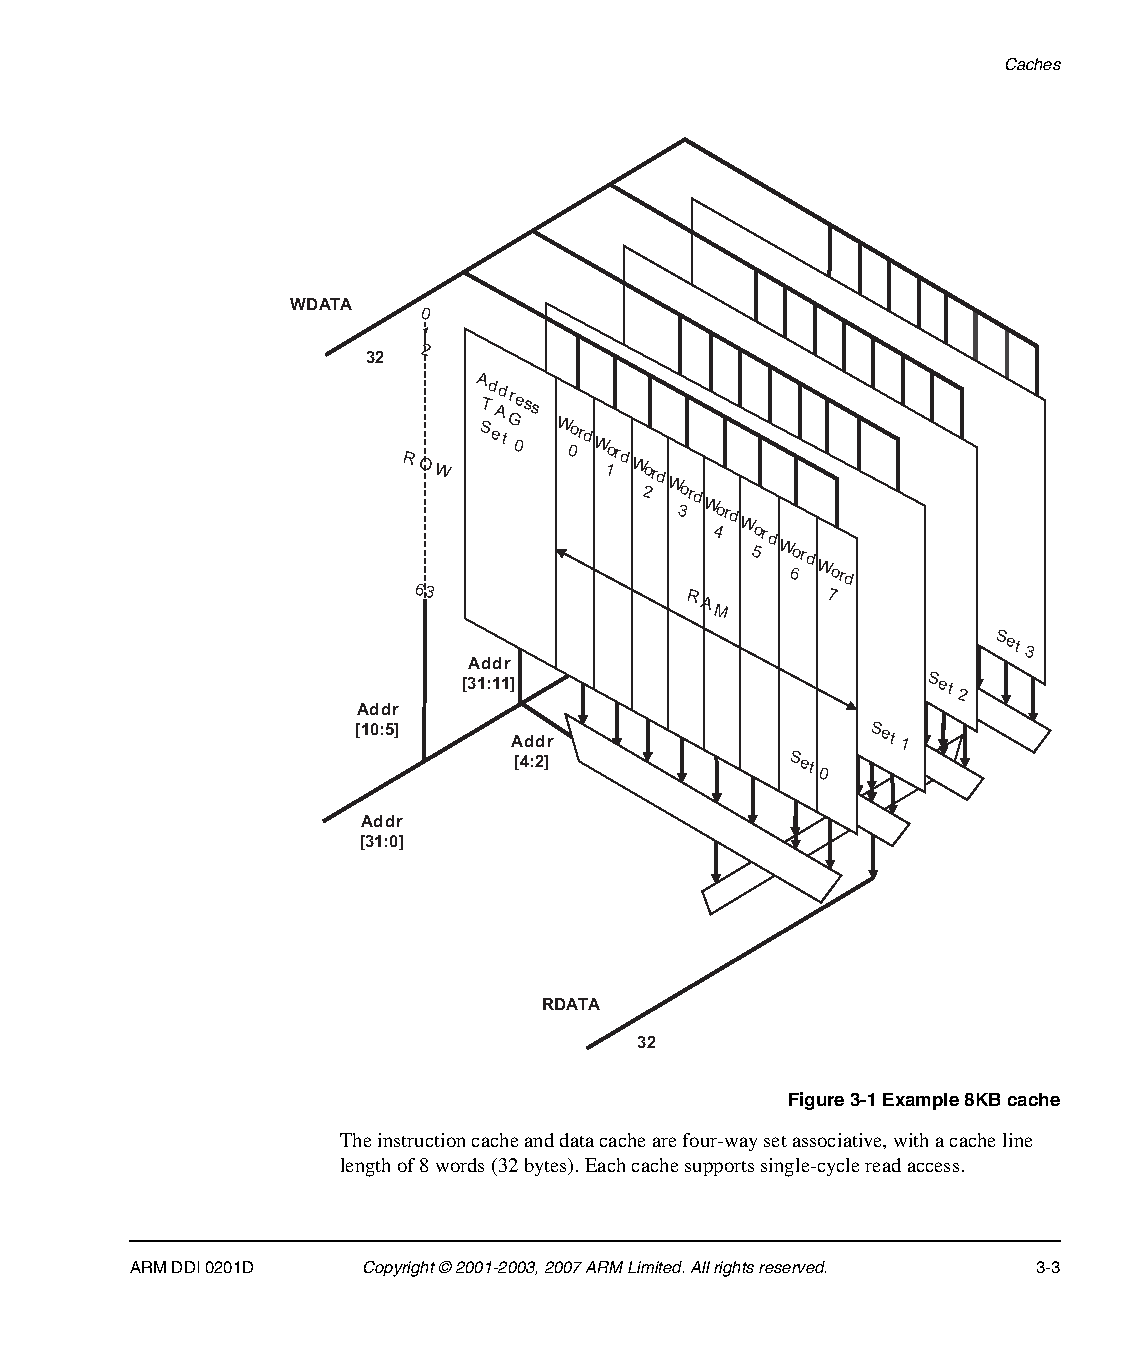
\includegraphics[clip,trim=4.5cm 5cm 1cm 2cm,width=\linewidth]{figures/icache.pdf}
		\caption{Instruction cache architecture of the DS ARM 9 \cite{arm946es_trm}.}
		\label{fig:icache}
	\end{figure}

	The instruction cache is controlled by the following CP15 instructions:
	\begin{description}
		\item[\texttt{mcr p15, 0, Rd, c7 , c5 , 0}] Invalidate (ARM: flush) entire instruction cache. \texttt{Rd} should be \texttt{0}.
		\item[\texttt{mcr p15, 0, Rd, c7 , c5 , 1}] Invalidate instruction cache line at address specified by \texttt{Rd}.
		\item[\texttt{mcr p15, 0, Rd, c7 , c13, 1}] Prefetch instruction cache line at address specified by \texttt{Rd}.
		\item[\texttt{mcr p15, 0, Rd, c9 , c0 , 1}] Write \textit{Instruction Lockdown Register}.
		\item[\texttt{mrc p15, 0, Rd, c9 , c0 , 1}] Read \textit{Instruction Lockdown Register}.
		\item[\texttt{mcr p15, 3, Rd, c15, c0 , 0}] Write \textit{Cache Debug Index Register}.
		\item[\texttt{mrc p15, 3, Rd, c15, c0 , 0}] Read \textit{Cache Debug Index Register}.
		\item[\texttt{mcr p15, 3, Rd, c15, c1 , 0}] Instruction TAG write.
		\item[\texttt{mrc p15, 3, Rd, c15, c1 , 0}] Instruction TAG read.
		\item[\texttt{mcr p15, 3, Rd, c15, c3 , 0}] Instruction cache write.
		\item[\texttt{mrc p15, 3, Rd, c15, c3 , 0}] Instruction cache read.
	\end{description}

	For cache mapping especially the debug instructions are important. They allow us to alter the contents of the cache; in particular the TAG that specifies the upper part of the memory address a cache line belongs to. This makes it possible to have the cache contain instructions at a memory location where those instructions do not actually exist. To prevent these mapped instructions from being evicted from the cache, this must be combined with locking down the part of the cache the mapped instructions are in.
	
	\subsubsection{How it works}
	The steps to map code are as follows:
	\begin{enumerate}
		\item First a 4 kB MPU region is setup at the target address. It should only allow instruction fetches, and have instruction cache enabled.
		
		\item Next the instruction cache is switched in lockdown mode by writing to the CP15 \textit{Instruction Lockdown Register}.
		
		\item The instructions are now loaded into the cache. When the source instructions are 2 kB aligned they can be quickly loaded into the cache using the instruction cache prefetch CP15 instruction (combined with the load flag in the \textit{Instruction Lockdown Register}). Otherwise, they must be written into the cache manually using the instruction cache write debug CP15 instruction. The reason for this is that part of the address determines the line index in the cache set (see Figure \ref{fig:icacheAddress}). When the source alignment is not right, the instructions will not end up at the right target address.
		
		\item Finally the TAG of the loaded cache lines must be adjusted to contain the intended target address. This is done using the Instruction TAG write CP15 instruction. Note that this can be interleaved with loading the instructions into the cache.
	\end{enumerate}
	It is important to note that when the CP15 instruction is used to invalidate the entire instruction cache, this also invalidates the locked parts of the cache. When this happens, either the TAGs must be fixed up manually, or the cache mapping must be disabled by disabling cache lockdown and the protection region.
	
	To map larger areas of memory the steps outlined above should be combined with a prefetch abort handler that will map the right chunk every time a jump outside the chunk is made. Note that additionally a data abort handler should be used, because data fetches cannot come from the instruction cache. The abort handler should take care to not read the aborted instruction with a regular load instruction as it will not fetch the right data. Instead the instruction can be read from the instruction cache with a debug CP15 instruction, or loaded from a different place in memory.
	
	\subsubsection{Impact of the solution}
	Pros:
	\begin{itemize}
		\item Makes it possible to run code in dynamically loaded chunks.
		\item You can run code at the originally intended address (for example the 0x08000000 region for GBA roms), which prevents relocation issues.
		\item No patches or modifications of the code are required.
		\item It was shown to fix games and rom hacks in practice on DSi and 3DS.
	\end{itemize}
	Cons:
	\begin{itemize}
		\item Only one 4 kB chunk can be loaded at a time.
		\item Cannot map a chunk smaller than 4 kB, because 4 kB is the minimum size of a protection region.
		\item While cache mapping is active half of the instruction cache is unusable for other memory regions.
		\item Loading of a 4 kB chunk is slow. When a lot of code is executed with this method, there is a significant performance degradation. Worst case is a loop at a 4 kB boundary. Best performance is achieved if the source instructions are 2 kB aligned such that instruction prefetch can be used. The performance issue is slightly mitigated by the fact that the code runs directly from the cache and can run at maximum CPU speed.
		\item All pool reads must be aborted.
		\item Special case required in the data abort handler to fetch the aborted instruction from the instruction cache.
		\item When a mix of linearly loaded instructions and cache mapping is used, it is still necessary to be able to disambiguate relative jumps from the linear to the dynamic part.
	\end{itemize}
	
	\subsection{Solution: JIT}
	When branches and pc-relative instructions are controlled by a JIT it becomes possible to run smaller chunks of code in a dynamic JIT cache.
	
	\subsubsection{Impact of the solution}
	Pros:
	\begin{itemize}
		\item 
	\end{itemize}
	Cons:
	\begin{itemize}
		\item 
	\end{itemize}

\section{Graphics compatibility issues}
	\subsection{GBA bitmap modes 3, 4 and 5 stride}
	\subsubsection{Solution: Special affine matrix}
	
	\subsection{GBA bitmap modes 3 and 5 alpha bit}
	\subsection{Sprite priorities}

\section{Sound issues}
	\subsection{ARM 7 cannot access sample data in IWRAM}
	

\chapter{System overview}
	In this chapter an overview will be given of the GBARunner 3 system, including block diagrams and memory maps.
	\newpage
	\section{Memory map}
	\subsection{ARM 9}
	\begin{figure}[htb]
		\centering
		\begin{minipage}[t]{0.5\linewidth}%
			\hspace{-0.75cm}%
			\begin{bytefield}{24}
				\memsection{05FFFFFF}{05000800}{4}{Palette Mirrors}\\
				\memsection{050007FF}{05000600}{2}{Sub OBJ Palette (0.5 KB)}\\
				\memsection{050005FF}{05000400}{2}{Sub BG Palette (0.5 KB)}\\
				\memsection{050003FF}{05000200}{2}{GBA OBJ Palette (0.5 KB)}\\
				\memsection{050001FF}{05000000}{2}{GBA BG Palette (0.5 KB)}\\
				\memsection{04FFFFFF}{04000000}{4}{IO Registers}\\
				\memsection{03FFFFFF}{03008000}{4}{GBA IWRAM Mirrors}\\
				\memsection{03007FFF}{03000000}{2}{GBA IWRAM (32 KB)}\\
				\memsection{02FFFFFF}{02400000}{4}{Main Memory Mirrors}\\
				\memsection{023FFFFF}{02200000}{2}{JIT (linear 2 MB)}\\
				\memsection{021FFFFF}{021C0000}{2}{JIT (dynamic 256 KB)}\\
				\memsection{021BFFFF}{020C0000}{2}{SD Cache (1 MB)}\\
				\memsection{020BFFFF}{020A0000}{2}{Save (128 KB)}\\
				\memsection{0209FFFF}{02040000}{2}{GBARunner 3 Data (384 KB)}\\
				\memsection{0203FFFF}{02000000}{2}{GBA EWRAM (256 KB)}\\
				\memsection{01FFFFFF}{00008000}{4}{Unmapped}\\
				\memsection{00007FFF}{00000000}{2}{ITCM (32 KB)}
			\end{bytefield}
		\end{minipage}%
		\begin{minipage}[t]{0.5\linewidth}%
			\hspace{-0.75cm}%
			\begin{bytefield}{24}
				\memsection{FFFFFFFF}{FFFFC000}{2}{DTCM (16 KB)}\\
				\memsection{FFFFBFFF}{80000000}{4}{DTCM Mirrors}\\
				\memsection{7FFFFFFF}{08000000}{4}{Unmapped}\\
				\memsection{07FFFFFF}{07000800}{3}{OAM Mirrors}\\
				\memsection{070007FF}{07000400}{2}{Sub OAM (1 KB)}\\
				\memsection{070003FF}{07000000}{2}{GBA OAM (1 KB)}\\
				\memsection{}{}{2}{}\\
				\memsection{0683FFFF}{06820000}{2}{LCDC VRAM B (128 KB)}\\
				\memsection{0682FFFF}{06800000}{2}{LCDC VRAM A (128 KB)}\\
				\memsection{067FFFFF}{06600000}{3}{Sub OBJ VRAM}\\
				\memsection{065FFFFF}{06408000}{3}{Main OBJ VRAM Mirrors}\\
				\memsection{06407FFF}{06404000}{2}{GBA OBJ VRAM (G, 16 KB)}\\
				\memsection{06403FFF}{06400000}{2}{GBA OBJ VRAM (F, 16 KB)\footnote{For BG modes 0, 1 and 2}}\\
				\memsection{063FFFFF}{06200000}{3}{Sub BG VRAM}\\
				\memsection{061FFFFF}{06014000}{3}{Main BG VRAM Mirrors}\\
				\memsection{06013FFF}{06010000}{2}{GBA BG VRAM (F, 16 KB)\footnote{For BG modes 3, 4 and 5}}\\
				\memsection{0600FFFF}{06000000}{2}{GBA BG VRAM (E, 64 KB)}
			\end{bytefield}
		\end{minipage}%
		\caption{Physical ARM 9 memory map for GBARunner 3 running on regular DS hardware.}
	\end{figure}

	\section{Memory protection regions}
		Regions with a higher index take priority over regions with a lower index. When the ARM 9 is running in non-privileged user mode the rights from the ``user" column apply, when running in a privileged mode the rights from the ``system" column apply.
		\begin{table}[htb]
			\centering
			\begin{tabular}{l|l|l|l|l|l}
				\# & region & description & user & system & cache \& wrbuf \\ \hline
				7 & \texttt{02000000-0203FFFF} & GBA EWRAM & \texttt{R/W/X} & \texttt{R/W/X} & \texttt{i/-/-} \\
				6 & \texttt{03000000-03FFFFFF} & GBA IWRAM & \texttt{R/W/X} & \texttt{R/W/X} & \texttt{i/-/-} \\
				5 & \texttt{06800000-0683FFFF} & LCDC VRAM A, B & \texttt{-/-/-} & \texttt{R/W/X} & \texttt{i/d/wrbuf} \\
				2 & \texttt{06000000-067FFFFF} & VRAM & \texttt{R/-/X} & \texttt{R/W/X} & \texttt{i/-/-} \\
				1 & \texttt{02000000-023FFFFF} & Main Memory & \texttt{R/-/X} & \texttt{R/W/X} & \texttt{i/d/wrbuf} \\
				0 & \texttt{00000000-FFFFFFFF} & ITCM, DTCM, uncached mmem, IO & \texttt{-/-/-} & \texttt{R/W/X} & \texttt{-/-/-}
			\end{tabular}
			\caption{Overview of the memory protection regions for GBARunner 3.}			
		\end{table}
	
\chapter{Virtual machine}\label{chap_vm}
	To have more control over the running game GBARunner 3 will use a Virtual Machine (hereafter VM) in which the GBA code runs. All code inside the VM will run in user mode (non-privileged). The actual mode of the virtualized ARM core will be held in the state of the VM. An additional advantage of this is that emulating aborted memory access instructions is easier when all code runs in user mode. By using the VM the GBA code will not be able to fully turn off interrupts by using the CPSR I bit. In such a case the VM will not receive any interrupts, but interrupts that are essential for the functioning of GBARunner 3 can still be handled.
	
	\section{Sensitive Instructions}
	Sensitive instructions are instructions that can change the state of the virtualized processor and that the VM needs to emulate. For GBA code there are no sensitive Thumb instructions. The following ARM instructions are sensitive:
	\begin{description}[leftmargin=!,labelwidth=4.5cm]
		\item[\texttt{mrs reg, cpsr}] Needs to read the CPSR from the VM state (combined with flags in the actual CPSR register).
		\item[\texttt{mrs reg, spsr}] Needs to read the SPSR from the VM state.
		\item[\texttt{msr cpsr, ...}] When a MSR instruction changes any of the control bits the change needs to be emulated by the VM.
		\item[\texttt{msr spsr, ...}] Needs to write the SPSR in the VM state.
		\item[\texttt{\textit{ALU}s pc, ...}] The SPSR to CPSR copy needs to be emulated by the VM.
		\item[\texttt{ldm\textit{XX} reg, \{...\}\textasciicircum}] Loading to user mode registers needs to be emulated by the VM.
		\item[\texttt{stm\textit{XX} reg, \{...\}\textasciicircum}] Storing from user mode registers needs to be emulated by the VM.
		\item[\texttt{ldm\textit{XX} reg, \{..., pc\}\textasciicircum}] The SPSR to CPSR copy needs to be emulated by the VM.
	\end{description}
	Because none of these instructions will cause an exception when executed in user mode they need to be replaced by exception generating instructions. This will be the task of the JIT (see Chapter \ref{chap_jit}).
	
	\section{Undefined instructions}
	To emulate sensitive instructions the VM will support undefined instructions that are drop-in replacements for the instructions. Additionally, the VM will support undefined instructions for unresolved branches.
	
	\begin{table}[htb]
		\begin{adjustbox}{center}
			\texttt{
				\arrayrulecolor{black}
				\begin{NiceTabular}{l|clll|cccccccccccccccccccccccccccc|}[colortbl-like]
					\hline
					MSR                        & \multicolumn{4}{c|}{}                                                                         & 0                         & \multicolumn{1}{c|}{0}    & \multicolumn{1}{c|}{I}                         & 1                                              & \multicolumn{1}{c|}{0}                         & \multicolumn{1}{c|}{R}                         & 1                         & \multicolumn{1}{c|}{0}                         & \multicolumn{1}{c|}{F} & \multicolumn{1}{c|}{S} & \multicolumn{1}{c|}{X} & \multicolumn{1}{c|}{C} & 1                      & 1                      & 1                      & \multicolumn{1}{c|}{1} & \multicolumn{12}{c|}{2nd op}                                                                                                                                                                                                                                                                                                                                          \\ \cline{1-1} \cline{6-33} 
					& \multicolumn{4}{c|}{}                                                                         & \cellcolor[HTML]{C0C0C0}0 & \cellcolor[HTML]{C0C0C0}0 & \cellcolor[HTML]{C0C0C0}0                      & \cellcolor[HTML]{C0C0C0}1                      & \multicolumn{1}{c|}{\cellcolor[HTML]{C0C0C0}1} & \multicolumn{1}{c|}{R}                         & \multicolumn{1}{c|}{0}    & \multicolumn{1}{c|}{I}                         & \multicolumn{12}{c|}{2nd op}                                                                                                                                                                                                                                                                                                                              & \cellcolor[HTML]{C0C0C0}1 & \cellcolor[HTML]{C0C0C0}0 & \cellcolor[HTML]{C0C0C0}0 & \multicolumn{1}{c|}{\cellcolor[HTML]{C0C0C0}1} & \multicolumn{1}{c|}{F} & \multicolumn{1}{c|}{S} & \multicolumn{1}{c|}{X} & C \\ \cline{1-1} \cline{6-33} 
					MRS                        & \multicolumn{4}{c|}{}                                                                         & 0                         & 0                         & 0                                              & 1                                              & \multicolumn{1}{c|}{0}                         & \multicolumn{1}{c|}{R}                         & 0                         & 0                                              & 0                      & 0                      & 0                      & \multicolumn{1}{c|}{0} & \multicolumn{4}{c|}{Rd}                                                                           & 0                                              & 0                      & 0                                              & 0                      & 0                         & 0                         & 0                         & 0                                              & 0                      & 0                      & 0                      & 0 \\ \cline{1-1} \cline{6-33} 
					& \multicolumn{4}{c|}{}                                                                         & \cellcolor[HTML]{C0C0C0}0 & \cellcolor[HTML]{C0C0C0}0 & \cellcolor[HTML]{C0C0C0}0                      & \cellcolor[HTML]{C0C0C0}1                      & \multicolumn{1}{c|}{\cellcolor[HTML]{C0C0C0}1} & \multicolumn{1}{c|}{R}                         & 1                         & 0                                              & 0                      & 0                      & 0                      & \multicolumn{1}{c|}{0} & \multicolumn{4}{c|}{Rd}                                                                           & 0                                              & 0                      & 0                                              & \multicolumn{1}{c|}{0} & \cellcolor[HTML]{C0C0C0}1 & \cellcolor[HTML]{C0C0C0}0 & \cellcolor[HTML]{C0C0C0}0 & \multicolumn{1}{c|}{\cellcolor[HTML]{C0C0C0}1} & 0                      & 0                      & 0                      & 0 \\ \cline{1-1} \cline{6-33} 
					LDM\textasciicircum (usr)  & \multicolumn{4}{c|}{}                                                                         & 1                         & 0                         & \multicolumn{1}{c|}{0}                         & \multicolumn{1}{c|}{P}                         & \multicolumn{1}{c|}{U}                         & 1                                              & 0                         & \multicolumn{1}{c|}{1}                         & \multicolumn{4}{c|}{Rn}                                                                           & \multicolumn{1}{c|}{0} & \multicolumn{15}{c|}{rlist}                                                                                                                                                                                                                                                                                                                                                                                                                      \\ \cline{1-1} \cline{6-33} 
					& \multicolumn{4}{c|}{}                                                                         & \cellcolor[HTML]{C0C0C0}0 & \cellcolor[HTML]{C0C0C0}0 & \cellcolor[HTML]{C0C0C0}1                      & \cellcolor[HTML]{C0C0C0}1                      & \multicolumn{1}{c|}{\cellcolor[HTML]{C0C0C0}0} & \multicolumn{1}{c|}{P}                         & \cellcolor[HTML]{C0C0C0}0 & \multicolumn{1}{c|}{\cellcolor[HTML]{C0C0C0}0} & \multicolumn{4}{c|}{Rn}                                                                           & \multicolumn{1}{c|}{U} & \multicolumn{15}{c|}{rlist}                                                                                                                                                                                                                                                                                                                                                                                                                      \\ \cline{1-1} \cline{6-33} 
					LDM\textasciicircum \{pc\} & \multicolumn{4}{c|}{}                                                                         & 1                         & 0                         & \multicolumn{1}{c|}{0}                         & \multicolumn{1}{c|}{P}                         & \multicolumn{1}{c|}{U}                         & \multicolumn{1}{c|}{1}                         & \multicolumn{1}{c|}{W}    & \multicolumn{1}{c|}{1}                         & \multicolumn{4}{c|}{Rn}                                                                           & \multicolumn{1}{c|}{1} & \multicolumn{15}{c|}{rlist}                                                                                                                                                                                                                                                                                                                                                                                                                      \\ \cline{1-1} \cline{6-33} 
					& \multicolumn{4}{c|}{}                                                                         & \cellcolor[HTML]{C0C0C0}0 & \cellcolor[HTML]{C0C0C0}1 & \multicolumn{1}{c|}{\cellcolor[HTML]{C0C0C0}1} & \multicolumn{4}{c|}{Rn}                                                                                                                                                      & \multicolumn{1}{c|}{1}                         & \multicolumn{15}{c|}{rlist}                                                                                                                                                                                                                                                                                                                                                                                                                   & \multicolumn{1}{c|}{\cellcolor[HTML]{C0C0C0}1} & \multicolumn{1}{c|}{P} & \multicolumn{1}{c|}{U} & \multicolumn{1}{c|}{1} & W \\ \cline{1-1} \cline{6-33} 
					LDM \{pc\}                 & \multicolumn{4}{c|}{}                                                                         & 1                         & 0                         & \multicolumn{1}{c|}{0}                         & \multicolumn{1}{c|}{P}                         & \multicolumn{1}{c|}{U}                         & \multicolumn{1}{c|}{0}                         & \multicolumn{1}{c|}{W}    & \multicolumn{1}{c|}{1}                         & \multicolumn{4}{c|}{Rn}                                                                           & \multicolumn{1}{c|}{1} & \multicolumn{15}{c|}{rlist}                                                                                                                                                                                                                                                                                                                                                                                                                      \\ \cline{1-1} \cline{6-33} 
					& \multicolumn{4}{c|}{}                                                                         & \cellcolor[HTML]{C0C0C0}0 & \cellcolor[HTML]{C0C0C0}1 & \multicolumn{1}{c|}{\cellcolor[HTML]{C0C0C0}1} & \multicolumn{4}{c|}{Rn}                                                                                                                                                      & \multicolumn{1}{c|}{0}                         & \multicolumn{15}{c|}{rlist}                                                                                                                                                                                                                                                                                                                                                                                                                   & \multicolumn{1}{c|}{\cellcolor[HTML]{C0C0C0}1} & \multicolumn{1}{c|}{P} & \multicolumn{1}{c|}{U} & \multicolumn{1}{c|}{1} & W \\ \cline{1-1} \cline{6-33} 
					STM\textasciicircum{}      & \multicolumn{4}{c|}{}                                                                         & 1                         & 0                         & \multicolumn{1}{c|}{0}                         & \multicolumn{1}{c|}{P}                         & \multicolumn{1}{c|}{U}                         & 1                                              & 0                         & \multicolumn{1}{c|}{0}                         & \multicolumn{4}{c|}{Rn}                                                                           & \multicolumn{16}{c|}{rlist}                                                                                                                                                                                                                                                                                                                                                                                                                                               \\ \cline{1-1} \cline{6-33} 
					& \multicolumn{4}{c|}{}                                                                         & \cellcolor[HTML]{C0C0C0}0 & \cellcolor[HTML]{C0C0C0}1 & \multicolumn{1}{c|}{\cellcolor[HTML]{C0C0C0}1} & \multicolumn{4}{c|}{Rn}                                                                                                                                                      & \multicolumn{16}{c|}{rlist}                                                                                                                                                                                                                                                                                                                                                                                                                                                                    & \multicolumn{1}{c|}{\cellcolor[HTML]{C0C0C0}1} & \multicolumn{1}{c|}{P} & \multicolumn{1}{c|}{U} & 0                      & 0 \\ \cline{1-1} \cline{6-33} 
					STM Rn!                    & \multicolumn{4}{c|}{}                                                                         & 1                         & 0                         & \multicolumn{1}{c|}{0}                         & \multicolumn{1}{c|}{P}                         & \multicolumn{1}{c|}{U}                         & \multicolumn{1}{c|}{0}                         & \multicolumn{1}{c|}{1}    & \multicolumn{1}{c|}{0}                         & \multicolumn{4}{c|}{Rn}                                                                           & \multicolumn{16}{c|}{rlist}                                                                                                                                                                                                                                                                                                                                                                                                                                               \\ \cline{1-1} \cline{6-33} 
					& \multicolumn{4}{c|}{}                                                                         & \cellcolor[HTML]{C0C0C0}0 & \cellcolor[HTML]{C0C0C0}1 & \multicolumn{1}{c|}{\cellcolor[HTML]{C0C0C0}1} & \multicolumn{4}{c|}{Rn}                                                                                                                                                      & \multicolumn{16}{c|}{rlist}                                                                                                                                                                                                                                                                                                                                                                                                                                                                    & \multicolumn{1}{c|}{\cellcolor[HTML]{C0C0C0}1} & \multicolumn{1}{c|}{P} & \multicolumn{1}{c|}{U} & 0                      & 1 \\ \cline{1-1} \cline{6-33} 
					ALU Rd=pc                  & \multicolumn{4}{c|}{}                                                                         & 0                         & \multicolumn{1}{c|}{0}    & \multicolumn{1}{c|}{I}                         & \multicolumn{4}{c|}{op}                                                                                                                                                      & \multicolumn{1}{c|}{S}                         & \multicolumn{4}{c|}{Rn}                                                                           & \multicolumn{1}{c|}{1} & \multicolumn{1}{c|}{1} & \multicolumn{1}{c|}{1} & \multicolumn{1}{c|}{1} & \multicolumn{12}{c|}{2nd op}                                                                                                                                                                                                                                                                                                                                          \\ \cline{1-1} \cline{6-33} 
					& \multicolumn{4}{c|}{}                                                                         & \cellcolor[HTML]{C0C0C0}1 & \cellcolor[HTML]{C0C0C0}1 & \cellcolor[HTML]{C0C0C0}1                      & \multicolumn{1}{c|}{\cellcolor[HTML]{C0C0C0}0} & \multicolumn{1}{c|}{0}                         & \multicolumn{1}{c|}{I}                         & \multicolumn{1}{c|}{S}    & \multicolumn{4}{c|}{Rn}                                                                                                   & \multicolumn{12}{c|}{2nd op}                                                                                                                                                                                                                                                                                                                                       & \multicolumn{1}{c|}{\cellcolor[HTML]{C0C0C0}0} & \multicolumn{4}{c|}{op}                                                      \\ \cline{1-1} \cline{6-33} 
					ALU Rn=pc                  & \multicolumn{4}{c|}{}                                                                         & 0                         & \multicolumn{1}{c|}{0}    & \multicolumn{1}{c|}{I}                         & \multicolumn{4}{c|}{op}                                                                                                                                                      & \multicolumn{1}{c|}{S}                         & 1                      & 1                      & 1                      & \multicolumn{1}{c|}{1} & \multicolumn{4}{c|}{Rd}                                                                           & \multicolumn{12}{c|}{2nd op}                                                                                                                                                                                                                                                                                                                                          \\ \cline{1-1} \cline{6-33} 
					& \multicolumn{4}{c|}{}                                                                         & \cellcolor[HTML]{C0C0C0}1 & \cellcolor[HTML]{C0C0C0}1 & \cellcolor[HTML]{C0C0C0}1                      & \multicolumn{1}{c|}{\cellcolor[HTML]{C0C0C0}0} & \multicolumn{1}{c|}{1}                         & \multicolumn{1}{c|}{I}                         & \multicolumn{1}{c|}{S}    & \multicolumn{4}{c|}{Rd}                                                                                                   & \multicolumn{12}{c|}{2nd op}                                                                                                                                                                                                                                                                                                                                       & \multicolumn{1}{c|}{\cellcolor[HTML]{C0C0C0}0} & \multicolumn{4}{c|}{op}                                                      \\ \cline{1-1} \cline{6-33} 
					ALU Rm=pc                  & \multicolumn{4}{c|}{}                                                                         & 0                         & 0                         & \multicolumn{1}{c|}{0}                         & \multicolumn{4}{c|}{op}                                                                                                                                                      & \multicolumn{1}{c|}{S}                         & \multicolumn{4}{c|}{Rn}                                                                           & \multicolumn{4}{c|}{Rd}                                                                           & \multicolumn{8}{c|}{2nd op}                                                                                                                                                                                                                                                            & 1                      & 1                      & 1                      & 1 \\ \cline{1-1} \cline{6-33} 
					& \multicolumn{4}{c|}{}                                                                         & \cellcolor[HTML]{C0C0C0}1 & \cellcolor[HTML]{C0C0C0}1 & \cellcolor[HTML]{C0C0C0}1                      & \multicolumn{1}{c|}{\cellcolor[HTML]{C0C0C0}0} & \multicolumn{4}{c|}{Rd}                                                                                                                                                      & \multicolumn{8}{c|}{2nd op}                                                                                                                                                                           & \multicolumn{1}{c|}{\cellcolor[HTML]{C0C0C0}1} & \multicolumn{1}{c|}{S} & \multicolumn{1}{c|}{\cellcolor[HTML]{C0C0C0}0} & \multicolumn{4}{c|}{Rn}                                                                                    & \multicolumn{1}{c|}{\cellcolor[HTML]{C0C0C0}1} & \multicolumn{4}{c|}{op}                                                      \\ \cline{1-1} \cline{6-33} 
					B                          & \multicolumn{4}{c|}{}                                                                         & 1                         & 0                         & 1                                              & \multicolumn{1}{c|}{0}                         & \multicolumn{24}{c|}{offset}                                                                                                                                                                                                                                                                                                                                                                                                                                                                                                                                                                                                                                                                                                                                 \\ \cline{1-1} \cline{6-33} 
					& \multicolumn{4}{c|}{}                                                                         & \cellcolor[HTML]{C0C0C0}1 & \cellcolor[HTML]{C0C0C0}1 & \multicolumn{1}{c|}{\cellcolor[HTML]{C0C0C0}0} & \multicolumn{1}{c|}{0}                         & \multicolumn{24}{c|}{offset}                                                                                                                                                                                                                                                                                                                                                                                                                                                                                                                                                                                                                                                                                                                                 \\ \cline{1-1} \cline{6-33} 
					BL                         & \multicolumn{4}{c|}{}                                                                         & 1                         & 0                         & 1                                              & \multicolumn{1}{c|}{1}                         & \multicolumn{24}{c|}{offset}                                                                                                                                                                                                                                                                                                                                                                                                                                                                                                                                                                                                                                                                                                                                 \\ \cline{1-1} \cline{6-33} 
					& \multicolumn{4}{c|}{}                                                                         & \cellcolor[HTML]{C0C0C0}1 & \cellcolor[HTML]{C0C0C0}1 & \multicolumn{1}{c|}{\cellcolor[HTML]{C0C0C0}0} & \multicolumn{1}{c|}{1}                         & \multicolumn{24}{c|}{offset}                                                                                                                                                                                                                                                                                                                                                                                                                                                                                                                                                                                                                                                                                                                                 \\ \cline{1-1} \cline{6-33} 
					LDR Rn=pc                  & \multicolumn{4}{c|}{}                                                                         & 0                         & \multicolumn{1}{c|}{1}    & \multicolumn{1}{c|}{I}                         & \multicolumn{1}{c|}{1}                         & \multicolumn{1}{c|}{U}                         & 0                                              & 0                         & 1                                              & 1                      & 1                      & 1                      & \multicolumn{1}{c|}{1} & \multicolumn{4}{c|}{Rd}                                                                           & \multicolumn{12}{c|}{2nd op}                                                                                                                                                                                                                                                                                                                                          \\ \cline{1-1} \cline{6-33} 
					& \multicolumn{4}{c|}{}                                                                         & \cellcolor[HTML]{C0C0C0}0 & \cellcolor[HTML]{C0C0C0}0 & \cellcolor[HTML]{C0C0C0}0                      & \cellcolor[HTML]{C0C0C0}0                      & \cellcolor[HTML]{C0C0C0}0                      & \multicolumn{1}{c|}{\cellcolor[HTML]{C0C0C0}1} & \multicolumn{1}{c|}{I}    & \multicolumn{1}{c|}{U}                         & \multicolumn{12}{c|}{2nd op}                                                                                                                                                                                                                                                                                                                              & \cellcolor[HTML]{C0C0C0}1 & \cellcolor[HTML]{C0C0C0}0 & \cellcolor[HTML]{C0C0C0}0 & \multicolumn{1}{c|}{\cellcolor[HTML]{C0C0C0}1} & \multicolumn{4}{c|}{Rd}                                                      \\ \cline{1-1} \cline{6-33} 
					LDR Rd=pc                  & \multicolumn{4}{c|}{}                                                                         & 0                         & \multicolumn{1}{c|}{1}    & \multicolumn{1}{c|}{I}                         & \multicolumn{1}{c|}{P}                         & \multicolumn{1}{c|}{U}                         & \multicolumn{1}{c|}{0}                         & \multicolumn{1}{c|}{W}    & \multicolumn{1}{c|}{1}                         & \multicolumn{4}{c|}{Rn}                                                                           & 1                      & 1                      & 1                      & \multicolumn{1}{c|}{1} & \multicolumn{12}{c|}{2nd op}                                                                                                                                                                                                                                                                                                                                          \\ \cline{1-1} \cline{6-33} 
					& \multicolumn{4}{c|}{}                                                                         & \cellcolor[HTML]{C0C0C0}1 & \cellcolor[HTML]{C0C0C0}1 & \cellcolor[HTML]{C0C0C0}1                      & \multicolumn{1}{c|}{\cellcolor[HTML]{C0C0C0}0} & \multicolumn{12}{c|}{2nd op}                                                                                                                                                                                                                                                                                                                                                         & \multicolumn{1}{c|}{\cellcolor[HTML]{C0C0C0}0} & \multicolumn{1}{c|}{1} & \multicolumn{1}{c|}{I}                         & \multicolumn{1}{c|}{P} & \multicolumn{1}{c|}{U}    & \multicolumn{1}{c|}{0}    & \multicolumn{1}{c|}{W}    & \multicolumn{1}{c|}{\cellcolor[HTML]{C0C0C0}1} & \multicolumn{4}{c|}{Rn}                                                      \\ \cline{1-1} \cline{6-33} 
					LDRH                       & \multicolumn{4}{c|}{}                                                                         & 0                         & 0                         & \multicolumn{1}{c|}{0}                         & \multicolumn{1}{c|}{P}                         & \multicolumn{1}{c|}{U}                         & \multicolumn{1}{c|}{I}                         & \multicolumn{1}{c|}{W}    & \multicolumn{1}{c|}{1}                         & \multicolumn{4}{c|}{Rn}                                                                           & \multicolumn{4}{c|}{Rd}                                                                           & \multicolumn{4}{c|}{addr\_mode}                                                                                                                   & 1                         & 0                         & 1                         & \multicolumn{1}{c|}{1}                         & \multicolumn{4}{c|}{addr\_mode}                                              \\ \cline{1-1} \cline{6-33} 
					& \multicolumn{4}{c|}{}                                                                         & \cellcolor[HTML]{C0C0C0}1 & \cellcolor[HTML]{C0C0C0}1 & \cellcolor[HTML]{C0C0C0}1                      & \multicolumn{1}{c|}{\cellcolor[HTML]{C0C0C0}0} & \multicolumn{4}{c|}{addr\_mode}                                                                                                                                              & \multicolumn{4}{c|}{Rn}                                                                           & \multicolumn{4}{c|}{Rd}                                                                           & \multicolumn{1}{c|}{\cellcolor[HTML]{C0C0C0}0} & \multicolumn{1}{c|}{0} & \multicolumn{1}{c|}{P}                         & \multicolumn{1}{c|}{U} & \multicolumn{1}{c|}{I}    & \multicolumn{1}{c|}{W}    & \multicolumn{1}{c|}{0}    & \multicolumn{1}{c|}{\cellcolor[HTML]{C0C0C0}1} & \multicolumn{4}{c|}{addr\_mode}                                              \\ \cline{1-1} \cline{6-33} 
					LDRSH                      & \multicolumn{4}{c|}{}                                                                         & 0                         & 0                         & \multicolumn{1}{c|}{0}                         & \multicolumn{1}{c|}{P}                         & \multicolumn{1}{c|}{U}                         & \multicolumn{1}{c|}{I}                         & \multicolumn{1}{c|}{W}    & \multicolumn{1}{c|}{1}                         & \multicolumn{4}{c|}{Rn}                                                                           & \multicolumn{4}{c|}{Rd}                                                                           & \multicolumn{4}{c|}{addr\_mode}                                                                                                                   & 1                         & 1                         & 1                         & \multicolumn{1}{c|}{1}                         & \multicolumn{4}{c|}{addr\_mode}                                              \\ \cline{1-1} \cline{6-33} 
					& \multicolumn{4}{c|}{}                                                                         & \cellcolor[HTML]{C0C0C0}1 & \cellcolor[HTML]{C0C0C0}1 & \cellcolor[HTML]{C0C0C0}1                      & \multicolumn{1}{c|}{\cellcolor[HTML]{C0C0C0}0} & \multicolumn{4}{c|}{addr\_mode}                                                                                                                                              & \multicolumn{4}{c|}{Rn}                                                                           & \multicolumn{4}{c|}{Rd}                                                                           & \multicolumn{1}{c|}{\cellcolor[HTML]{C0C0C0}0} & \multicolumn{1}{c|}{0} & \multicolumn{1}{c|}{P}                         & \multicolumn{1}{c|}{U} & \multicolumn{1}{c|}{I}    & \multicolumn{1}{c|}{W}    & \multicolumn{1}{c|}{1}    & \multicolumn{1}{c|}{\cellcolor[HTML]{C0C0C0}1} & \multicolumn{4}{c|}{addr\_mode}                                              \\ \cline{1-1} \cline{6-33} 
					BX                         & \multicolumn{4}{c|}{}                                                                         & 0                         & 0                         & 0                                              & 1                                              & 0                                              & 0                                              & 1                         & 0                                              & 1                      & 1                      & 1                      & 1                      & 1                      & 1                      & 1                      & 1                      & 1                                              & 1                      & 1                                              & 1                      & 0                         & 0                         & 0                         & \multicolumn{1}{c|}{1}                         & \multicolumn{4}{c|}{Rm}                                                      \\ \cline{1-1} \cline{6-33} 
					& \multicolumn{4}{c|}{\multirow{-34}{*}{\begin{tabular}[c]{@{}c@{}}c\\ o\\ n\\ d\end{tabular}}} & \cellcolor[HTML]{C0C0C0}0 & \cellcolor[HTML]{C0C0C0}0 & \cellcolor[HTML]{C0C0C0}0                      & \cellcolor[HTML]{C0C0C0}1                      & \multicolumn{1}{c|}{\cellcolor[HTML]{C0C0C0}1} & 0                                              & 1                         & 1                                              & 0                      & 0                      & 0                      & 0                      & 0                      & 0                      & 0                      & 0                      & 0                                              & 0                      & 0                                              & \multicolumn{1}{c|}{0} & \cellcolor[HTML]{C0C0C0}1 & \cellcolor[HTML]{C0C0C0}0 & \cellcolor[HTML]{C0C0C0}0 & \multicolumn{1}{c|}{\cellcolor[HTML]{C0C0C0}1} & \multicolumn{4}{c|}{Rm}                                                      \\ \hline
			\end{NiceTabular}}
		\end{adjustbox}
		\caption{Overview of ARM instructions and their undefined substitutions emulated by the VM.
			\todo[inline]{TODO: Update this table. It is outdated.}}
	\end{table}
	
\chapter{JIT patcher}\label{chap_jit}
	The purpose of the JIT patcher (hereafter JIT) is primarily to support the VM by replacing sensitive instructions by exception generating substitutes. Additionally, the JIT can fix CPU compatibility issues, fix relocation related issues and make it possible to execute code in higher areas of the ROM (also referred to as hicode). To minimize the overhead of the JIT, a couple of megabytes of the ROM (depending on the amount of available memory) will still be linearly loaded into memory, as was the case in GBARunner 2. To allow code outside this linearly loaded region to run there will also be a dynamic JIT cache. About 80~90\% of the games can run entirely from about 2MB of linearly loaded rom data. In such games it may be possible to run Thumb code without any JIT patches. The only critical patches are the ARM sensitive instruction patches, to make the VM work correctly.
	
	\section{Dynamic JIT cache}
	
\chapter{Memory emulator}\label{chap_mememu}
	Various memory accesses need to be emulated to allow the GBA code to access the right data and registers. The ARM946E-S has no MMU (memory mapping unit), but it does have a MPU (memory protection unit) that can be used to protect up to 8 regions of memory. When a data abort happens the abort handler code emulates the memory instruction. The performance of the abort handler plays an important role in the performance of the entire system.
	\section{Memory Instructions}
	In this section an overview will be given of the instructions that need to be emulated.
	\subsection{ARM Memory Instructions}
	\begin{table}[htb]
		\begin{adjustbox}{center}
		\texttt{
		\arrayrulecolor{black}
		\begin{tabular}{l|c|ccc|c|c|c|c|c|c|c|ccccc|cc|c|c|}
		& \footnotesize 31 \quad 28 & \footnotesize 27 & \footnotesize 26 & \footnotesize 25 & \footnotesize 24 & \footnotesize 23 & \footnotesize 22 & \footnotesize 21 & \footnotesize 20 & \footnotesize 19 \quad 16 & \footnotesize 15 \quad 12 & \footnotesize 11 & \footnotesize 10 & \footnotesize 9 & \footnotesize 8 & \footnotesize 7 & \footnotesize 6 & \footnotesize 5 & \footnotesize 4 & \footnotesize 3 \qquad\qquad\quad 0 \\
		\hline
		SWP                                                          & \multirow{16}{*}{cond} & \multirow{2}{*}{0}                   & \multirow{2}{*}{0}                                        & \multicolumn{1}{c}{\multirow{2}{*}{0}}                  & \multicolumn{1}{c}{\multirow{2}{*}{1}} & \multirow{2}{*}{0}  & 0                                                       & \multicolumn{1}{c}{\multirow{2}{*}{0}} & \multirow{2}{*}{0}                   & \multirow{16}{*}{Rn} & \multirow{14}{*}{Rd} & \multirow{2}{*}{0} & \multirow{2}{*}{0} & \multirow{2}{*}{0} & \multirow{2}{*}{0}     & \multicolumn{1}{c}{\multirow{2}{*}{1}}                   & \multirow{2}{*}{0}                   & \multicolumn{1}{c}{\multirow{2}{*}{0}}                   & \multirow{2}{*}{1}                   & \multirow{2}{*}{Rm}                                               \\ 
		\cline{1-1}\cline{8-8}
		SWPB                                                         &                        &                                      &                                                           & \multicolumn{1}{c}{}                                    & \multicolumn{1}{c}{}                   &                     & 1                                                       & \multicolumn{1}{c}{}                   &                                      &                      &                      &                    &                    &                    &                        & \multicolumn{1}{c}{}                                     &                                      & \multicolumn{1}{c}{}                                     &                                      &                                                                   \\ 
		\hhline{-~--------~~---------|}
		STRH                                                         &                        & \multirow{4}{*}{0}                   & \multirow{4}{*}{0}                                        & \multirow{4}{*}{0}                                      & \multirow{12}{*}{P}                    & \multirow{12}{*}{U} & {\cellcolor[rgb]{0.502,0.502,0.502}}                    & \multirow{12}{*}{W}                    & 0                                    &                      &                      & \multicolumn{4}{c|}{{\cellcolor[rgb]{0.502,0.502,0.502}}}                             & \multirow{4}{*}{1}                                       & \multirow{2}{*}{0}                   & \multirow{2}{*}{1}                                       & \multirow{4}{*}{1}                   & {\cellcolor[rgb]{0.502,0.502,0.502}}                              \\ 
		\hhline{-~~~~~~>{\arrayrulecolor[rgb]{0.502,0.502,0.502}}-~>{\arrayrulecolor{black}}-~~>{\arrayrulecolor[rgb]{0.502,0.502,0.502}}----~~~~->{\arrayrulecolor{black}}|}
		LDRH                                                         &                        &                                      &                                                           &                                                         &                                        &                     & {\cellcolor[rgb]{0.502,0.502,0.502}}                    &                                        & \multirow{3}{*}{1}                   &                      &                      & \multicolumn{4}{c|}{{\cellcolor[rgb]{0.502,0.502,0.502}}}                             &                                                          &                                      &                                                          &                                      & {\cellcolor[rgb]{0.502,0.502,0.502}}                              \\ 
		\hhline{-~~~~~~>{\arrayrulecolor[rgb]{0.502,0.502,0.502}}-~~~~----~>{\arrayrulecolor{black}}--~>{\arrayrulecolor[rgb]{0.502,0.502,0.502}}->{\arrayrulecolor{black}}|}
		LDRSB                                                        &                        &                                      &                                                           &                                                         &                                        &                     & {\cellcolor[rgb]{0.502,0.502,0.502}}                    &                                        &                                      &                      &                      & \multicolumn{4}{c|}{{\cellcolor[rgb]{0.502,0.502,0.502}}}                             &                                                          & 1                                    & 0                                                        &                                      & {\cellcolor[rgb]{0.502,0.502,0.502}}                              \\ 
		\hhline{-~~~~~~>{\arrayrulecolor[rgb]{0.502,0.502,0.502}}-~~~~----~>{\arrayrulecolor{black}}--~>{\arrayrulecolor[rgb]{0.502,0.502,0.502}}->{\arrayrulecolor{black}}|}
		LDRSH                                                        &                        &                                      &                                                           &                                                         &                                        &                     & \multirow{-4}{*}{{\cellcolor[rgb]{0.502,0.502,0.502}}I} &                                        &                                      &                      &                      & \multicolumn{4}{c|}{\multirow{-4}{*}{{\cellcolor[rgb]{0.502,0.502,0.502}}addr\_mode}} &                                                          & 1                                    & 1                                                        &                                      & \multirow{-4}{*}{{\cellcolor[rgb]{0.502,0.502,0.502}}addr\_mode}  \\ 
		\hhline{-~---~~-~-~~---------|}
		\multicolumn{1}{r|}{{\cellcolor[rgb]{0.502,0.502,0.502}}reg} &                        & {\cellcolor[rgb]{0.502,0.502,0.502}} & {\cellcolor[rgb]{0.502,0.502,0.502}}                      & {\cellcolor[rgb]{0.502,0.502,0.502}}                    &                                        &                     & 0                                                       &                                        & {\cellcolor[rgb]{0.502,0.502,0.502}} &                      &                      & 0                  & 0                  & 0                  & \multicolumn{1}{c|}{0} & \multicolumn{1}{c}{{\cellcolor[rgb]{0.502,0.502,0.502}}} & {\cellcolor[rgb]{0.502,0.502,0.502}} & \multicolumn{1}{c}{{\cellcolor[rgb]{0.502,0.502,0.502}}} & {\cellcolor[rgb]{0.502,0.502,0.502}} & Rm                                                                \\ 
		\hhline{>{\arrayrulecolor[rgb]{0.502,0.502,0.502}}-~---~~>{\arrayrulecolor{black}}-~>{\arrayrulecolor[rgb]{0.502,0.502,0.502}}-~~>{\arrayrulecolor{black}}---->{\arrayrulecolor[rgb]{0.502,0.502,0.502}}---->{\arrayrulecolor{black}}-|}
		\multicolumn{1}{r|}{{\cellcolor[rgb]{0.502,0.502,0.502}}imm} &                        & {\cellcolor[rgb]{0.502,0.502,0.502}} & {\cellcolor[rgb]{0.502,0.502,0.502}}                      & {\cellcolor[rgb]{0.502,0.502,0.502}}                    &                                        &                     & 1                                                       &                                        & {\cellcolor[rgb]{0.502,0.502,0.502}} &                      &                      & \multicolumn{4}{c|}{immH}                                                             & \multicolumn{1}{c}{{\cellcolor[rgb]{0.502,0.502,0.502}}} & {\cellcolor[rgb]{0.502,0.502,0.502}} & \multicolumn{1}{c}{{\cellcolor[rgb]{0.502,0.502,0.502}}} & {\cellcolor[rgb]{0.502,0.502,0.502}} & immL                                                              \\ 
		\hhline{-~---~~-~-~~---------|}
		STR                                                          &                        & \multirow{4}{*}{0}                   & \multicolumn{1}{c|}{\multirow{4}{*}{1}}                   & {\cellcolor[rgb]{0.502,0.502,0.502}}                    &                                        &                     & \multirow{2}{*}{0}                                      &                                        & 0                                    &                      &                      & \multicolumn{9}{c|}{{\cellcolor[rgb]{0.502,0.502,0.502}}}                                                                                                                                                                                                                                                                                                     \\ 
		\hhline{-~~~>{\arrayrulecolor[rgb]{0.502,0.502,0.502}}-~~~~>{\arrayrulecolor{black}}-~~>{\arrayrulecolor[rgb]{0.502,0.502,0.502}}--------->{\arrayrulecolor{black}}|}
		LDR                                                          &                        &                                      & \multicolumn{1}{c|}{}                                     & {\cellcolor[rgb]{0.502,0.502,0.502}}                    &                                        &                     &                                                         &                                        & 1                                    &                      &                      & \multicolumn{9}{c|}{{\cellcolor[rgb]{0.502,0.502,0.502}}}                                                                                                                                                                                                                                                                                                     \\ 
		\hhline{-~~~>{\arrayrulecolor[rgb]{0.502,0.502,0.502}}-~~>{\arrayrulecolor{black}}-~-~~>{\arrayrulecolor[rgb]{0.502,0.502,0.502}}--------->{\arrayrulecolor{black}}|}
		STRB                                                         &                        &                                      & \multicolumn{1}{c|}{}                                     & {\cellcolor[rgb]{0.502,0.502,0.502}}                    &                                        &                     & \multirow{2}{*}{1}                                      &                                        & 0                                    &                      &                      & \multicolumn{9}{c|}{{\cellcolor[rgb]{0.502,0.502,0.502}}}                                                                                                                                                                                                                                                                                                     \\ 
		\hhline{-~~~>{\arrayrulecolor[rgb]{0.502,0.502,0.502}}-~~~~>{\arrayrulecolor{black}}-~~>{\arrayrulecolor[rgb]{0.502,0.502,0.502}}--------->{\arrayrulecolor{black}}|}
		LDRB                                                         &                        &                                      & \multicolumn{1}{c|}{}                                     & \multirow{-4}{*}{{\cellcolor[rgb]{0.502,0.502,0.502}}I} &                                        &                     &                                                         &                                        & 1                                    &                      &                      & \multicolumn{9}{c|}{\multirow{-4}{*}{{\cellcolor[rgb]{0.502,0.502,0.502}}addr\_mode}}                                                                                                                                                                                                                                                                         \\ 
		\hhline{-~---~~-~-~~---------|}
		\multicolumn{1}{r|}{{\cellcolor[rgb]{0.502,0.502,0.502}}imm} &                        & {\cellcolor[rgb]{0.502,0.502,0.502}} & \multicolumn{1}{c|}{{\cellcolor[rgb]{0.502,0.502,0.502}}} & 0                                                       &                                        &                     & {\cellcolor[rgb]{0.502,0.502,0.502}}                    &                                        & {\cellcolor[rgb]{0.502,0.502,0.502}} &                      &                      & \multicolumn{9}{c|}{offset\_12}                                                                                                                                                                                                                                                                                                                               \\ 
		\hhline{>{\arrayrulecolor[rgb]{0.502,0.502,0.502}}-~-->{\arrayrulecolor{black}}-~~>{\arrayrulecolor[rgb]{0.502,0.502,0.502}}-~-~~>{\arrayrulecolor{black}}---------|}
		\multicolumn{1}{r|}{{\cellcolor[rgb]{0.502,0.502,0.502}}reg} &                        & {\cellcolor[rgb]{0.502,0.502,0.502}} & \multicolumn{1}{c|}{{\cellcolor[rgb]{0.502,0.502,0.502}}} & 1                                                       &                                        &                     & {\cellcolor[rgb]{0.502,0.502,0.502}}                    &                                        & {\cellcolor[rgb]{0.502,0.502,0.502}} &                      &                      & \multicolumn{5}{c|}{shift\_imm}                                                                                                                  & \multicolumn{2}{c|}{shift}                                                                      & 0                                    & Rm                                                                \\ 
		\cline{1-1}\cline{3-10}\cline{12-21}
		STM                                                          &                        & \multirow{2}{*}{1}                   & \multirow{2}{*}{0}                                        & \multirow{2}{*}{0}                                      & \multirow{2}{*}{P}                     & \multirow{2}{*}{U}  & \multirow{2}{*}{0}                                      & \multirow{2}{*}{W}                     & 0                                    &                      & \multicolumn{10}{c|}{\multirow{2}{*}{register\_list}}                                                                                                                                                                                                                                                                                                                                \\ 
		\cline{1-1}\cline{10-10}
		LDM                                                          &                        &                                      &                                                           &                                                         &                                        &                     &                                                         &                                        & 1                                    &                      & \multicolumn{10}{c|}{}                                                                                                                                                                                                                                                                                                                                                               \\
		\hline
		\end{tabular}}
		\end{adjustbox}
		\caption{Overview of ARM memory instructions that could cause an abort.}
	\end{table}
	\subsection{Thumb Memory Instructions}
	\begin{table}[htb]
		\centering
		\texttt{
		\begin{tabular}{l|cccc|c|cc|cl|c|c|}
		& \footnotesize 15 & \footnotesize 14 & \footnotesize 13 & \footnotesize 12 & \footnotesize 11 & \footnotesize 10 & \footnotesize 9 & \footnotesize 8 & \footnotesize 7 \quad 6 & \footnotesize 5 \quad 3 & \footnotesize 2 \quad 0 \\
		\hline
		STR reg   & \multirow{8}{*}{0} & \multirow{8}{*}{1} & \multirow{8}{*}{0}                      & \multirow{8}{*}{1}    & \multicolumn{1}{c}{0} & 0                  & 0                  & \multicolumn{2}{c|}{\multirow{8}{*}{Rm}} & \multirow{14}{*}{Rn} & \multirow{14}{*}{Rd}  \\ 
		\cline{1-1}\cline{6-8}
		STRH reg  &                    &                    &                                         &                       & \multicolumn{1}{c}{0} & 0                  & 1                  &                                         &                   &                      &                       \\ 
		\cline{1-1}\cline{6-8}
		STRB reg  &                    &                    &                                         &                       & \multicolumn{1}{c}{0} & 1                  & 0                  &                                         &                   &                      &                       \\ 
		\cline{1-1}\cline{6-8}
		LDRSB reg &                    &                    &                                         &                       & \multicolumn{1}{c}{0} & 1                  & 1                  &                                         &                   &                      &                       \\ 
		\cline{1-1}\cline{6-8}
		LDR reg   &                    &                    &                                         &                       & \multicolumn{1}{c}{1} & 0                  & 0                  &                                         &                   &                      &                       \\ 
		\cline{1-1}\cline{6-8}
		LDRH reg  &                    &                    &                                         &                       & \multicolumn{1}{c}{1} & 0                  & 1                  &                                         &                   &                      &                       \\ 
		\cline{1-1}\cline{6-8}
		LDRB reg  &                    &                    &                                         &                       & \multicolumn{1}{c}{1} & 1                  & 0                  &                                         &                   &                      &                       \\ 
		\cline{1-1}\cline{6-8}
		LDRSH reg &                    &                    &                                         &                       & \multicolumn{1}{c}{1} & 1                  & 1                  &                                         &                   &                      &                       \\ 
		\cline{1-10}
		STR imm   & \multirow{4}{*}{0} & \multirow{4}{*}{1} & \multicolumn{1}{c|}{\multirow{4}{*}{1}} & \multirow{2}{*}{0}    & 0                     & \multicolumn{4}{c|}{\multirow{6}{*}{imm}}                                                             &                      &                       \\ 
		\cline{1-1}\cline{6-6}
		LDR imm   &                    &                    & \multicolumn{1}{c|}{}                   &                       & 1                     & \multicolumn{4}{c|}{}                                                                                 &                      &                       \\ 
		\cline{1-1}\cline{5-6}
		STRB imm  &                    &                    & \multicolumn{1}{c|}{}                   & \multirow{2}{*}{1}    & 0                     & \multicolumn{4}{c|}{}                                                                                 &                      &                       \\ 
		\cline{1-1}\cline{6-6}
		LDRB imm  &                    &                    & \multicolumn{1}{c|}{}                   &                       & 1                     & \multicolumn{4}{c|}{}                                                                                 &                      &                       \\ 
		\cline{1-6}
		STRH imm  & \multirow{2}{*}{1} & \multirow{2}{*}{0} & \multirow{2}{*}{0}                      & \multirow{2}{*}{0}    & 0                     & \multicolumn{4}{c|}{}                                                                                 &                      &                       \\ 
		\cline{1-1}\cline{6-6}
		LDRH imm  &                    &                    &                                         &                       & 1                     & \multicolumn{4}{c|}{}                                                                                 &                      &                       \\ 
		\hline
		LDR pc    & 0                  & 1                  & 0                                       & \multicolumn{1}{c}{0} & 1                     & \multicolumn{3}{c|}{\multirow{3}{*}{Rd}}                                          & \multicolumn{3}{c|}{\multirow{3}{*}{imm}}                        \\ 
		\cline{1-6}
		STR sp    & \multirow{2}{*}{1} & \multirow{2}{*}{0} & \multirow{2}{*}{0}                      & \multirow{2}{*}{1}    & 0                     & \multicolumn{3}{c|}{}                                                             & \multicolumn{3}{c|}{}                                            \\ 
		\cline{1-1}\cline{6-6}
		LDR sp    &                    &                    &                                         &                       & 1                     & \multicolumn{3}{c|}{}                                                             & \multicolumn{3}{c|}{}                                            \\ 
		\hline
		PUSH      & \multirow{2}{*}{1} & \multirow{2}{*}{0} & \multirow{2}{*}{1}                      & \multirow{2}{*}{1}    & 0                     & \multirow{2}{*}{1} & \multirow{2}{*}{0} & \multicolumn{1}{c|}{\multirow{2}{*}{R}} & \multicolumn{3}{c|}{\multirow{4}{*}{register\_list}}             \\ 
		\cline{1-1}\cline{6-6}
		POP       &                    &                    &                                         &                       & 1                     &                    &                    & \multicolumn{1}{c|}{}                   & \multicolumn{3}{c|}{}                                            \\ 
		\cline{1-9}
		STMIA     & \multirow{2}{*}{1} & \multirow{2}{*}{1} & \multirow{2}{*}{0}                      & \multirow{2}{*}{0}    & 0                     & \multicolumn{3}{c|}{\multirow{2}{*}{Rn}}                                          & \multicolumn{3}{c|}{}                                            \\ 
		\cline{1-1}\cline{6-6}
		LDMIA     &                    &                    &                                         &                       & 1                     & \multicolumn{3}{c|}{}                                                             & \multicolumn{3}{c|}{}                                            \\
		\hline
		\end{tabular}}
		\caption{Overview of Thumb memory instructions that could cause an abort.}
	\end{table}
\chapter{SD cache}
	GBARunner 2 used a least-recently-used (LRU) cache. Using a simpler replacement algorithm such as pseudo-random might be more efficient in practice, because LRU requires an update to the cache block list for every access.
\chapter{GBA peripherals emulation}
	\section{Graphics}
	\section{Timers}
	\section{Sound}
	\section{DMA}
	\section{SIO}
	
\clearpage
{
	\raggedright
	\printbibliography
}
\end{document}